\documentclass{article}
\usepackage{amsmath}
\usepackage[margin=0.5in]{geometry}
\usepackage{breakcites}
\usepackage{natbib}
\usepackage{mathtools}
\usepackage{mathrsfs}
\usepackage{graphicx}
\usepackage{caption}
\usepackage[bottom]{footmisc}
\usepackage[export]{adjustbox}
\usepackage{todonotes}
\usepackage{footnote}
\usepackage{threeparttable}
\usepackage{xr}
\externaldocument[S-]{supplement}
\DeclarePairedDelimiter\ceil{\lceil}{\rceil}
\DeclarePairedDelimiter\floor{\lfloor}{\rfloor}
\DeclareMathAlphabet\mathbfcal{OMS}{cmsy}{b}{n}
\DeclareMathOperator*{\argmin}{arg\,min}

\begin{document}


\newcommand{\monosaccharide}[1]{{\bf #1}}
\newcommand{\nglycan}[0]{\textit{N}-glycan }
\newcommand{\nglycans}[0]{\textit{N}-glycans }

\newcommand{\msn}[0]{$MS^n$}
\newcommand{\ms}[1]{$MS^#1$}

% Sample Name Shortcuts
\newcommand{\agp}[0]{\textit{20150930-06-AGP} }
\newcommand{\phil}[0]{\textit{20141031-07-Phil-82} }
\newcommand{\philbs}[0]{\textit{20141101-04-Phil-BS} }
\newcommand{\igg}[0]{\textit{20151002-02-IGG} }
\newcommand{\dpphil}[0]{\textit{20141128-11-Phil-82} }
\newcommand{\dpagp}[0]{\textit{AGP-DR-Perm-glycans-1} }
\newcommand{\rpagp}[0]{\textit{AGP-permethylated-2ul-inj-55-SLens} }
\newcommand{\rphumanserum}[0]{\textit{Perm-BS-070111-04-Human-Serum} }


\section{Chromatographic Feature Evaluation}\label{sec:feature_evaluation}
    For each candidate feature, we computed several statistics to estimate how distinguishable
    the observed signal was from random noise. We use the following quantities from each LC-MS
    feature:

    \renewcommand{\arraystretch}{1.5}
    \begin{table}
        \caption{Chromatogram Feature Definitions}\label{tbl:chromatogram_feature_definitions}
        \centering
        \begin{tabular}{l | p{9cm}}
            \hline
            $\mathcal{M}_i$ & The neutral mass of the $i$th chromatogram\\
            $\mathbfcal{I}_i$ & The total intensity array assigned to the $i$th chromatogram\\
            $\mathbfcal{I}_{i, j}$ & The sum of all peak intensities for peaks observed in
                                             the $j$th scan for the $i$th chromatogram\\
            $\mathcal{I}_{i, j, k}$ & The intensity assigned to the $k$th peak at the $j$th
                                      scan for the $i$th chromatogram\\
            $\mathbf{c}_i$ & The set of charge states observed for the $i$th chromatogram\\
            $\mathbfcal{I}_{i, c=j}$ & The total intensity assigned to the $i$th chromatogram
                                     with charge state $j$\\
            $\mathbf{t}_{i, j}$ & The time of the $j$th scan of the $i$th chromatogram\\
            $\textbf{env}_{i, j, k}$ & The normalized experimental isotopic envelope composing
                                     the $k$th peak of the $j$th scan of the $i$th chromatogram,
                                     whose members sum to $1$\\
            $\mathbf{a}_i$ & The set of adduction states observed for the $i$th chromatogram\\
            $\mathbfcal{I}_{i, a=j}$ & The total intensity assigned to the $i$th
                                                 chromatogram with adduct $j$\\
            ${\hat g}_i$ & The glycan composition assigned to the $i$th chromatogram, or \O
                           \ if there was no matched glycan composition
        \end{tabular}
    \end{table}
    \renewcommand{\arraystretch}{1.0}

    \subsubsection{Chromatographic Peak Shape}
        An LC-MS elution profile should be composed of one or more peak-like components, each
        following a bi-Gaussian peak shape model (\cite{Yu2010}) or in less ideal chromatographic
        circumstances, a skewed Gaussian peak shape model. We fit these models using non-linear
        least squares (NLS). As measures of goodness of fit are not generally available for NLS,
        we use the following criterion:
        \begin{align}
            {\hat y_i} &= NLS(\mathbfcal{I}_i, \mathbf{t}_i) \nonumber\\
            e_{i, NLS} &= \mathbfcal{I}_i - {\hat y_i} \nonumber\\
            {\bar y_i} &= \mathbf{t}_i
                \left(
                    \left(
                        \mathbf{t}_i^t\mathbf{t}_i
                    \right)^{-1}\mathbf{t}_i\mathbfcal{I}_i
                \right)\nonumber\\
            e_{i, null} &= \mathbfcal{I}_i - {\bar y_i} \nonumber\\
            \mathscr{L}_i &= 1 - \frac{\sum{e_{i, NLS}^2}}{\sum{e_{i, null}^2}}
        \end{align}
        \noindent where line score describes how much the peak shape fit improves on a straight
        line fit null model.

        % Likely to be moved to the supplement
        We apply two competitive peak fitting strategies to address distorted, overlapping, or
        multimodal elution profiles. The first works iteratively by finding a best-matching peak
        shape using non-linear least squares, subtracting the fitted signal and checks if there is
        another peak with at least half as tall as the removed peak, if so repeating the process until
        no peak can be found, saving each peak model so constructed. The second approach starts
        by locating local minima between putative peaks, and partitioning the chromatogram into
        sub-groups which would are fit independently. This method generates a candidate list of
        minima, and selects the case which has the greatest difference between the minimum and its
        pair of maxima to split the feature at. The strategy which produces the maximum $\mathscr{L}_i$
        is chosen.

    \subsubsection{Composition Dependent Charge State Distribution}
        % Does this principle need a citation?
        As the number of monosaccharides composing a glycan increases, the number of possible sites
        for charge localization increases. Under normal conditions, we would expect to observe the
        same molecule in multiple charge states (\cite{Maxwell2012}). Which charge states are
        expected would depend upon the size of the molecule and it's constituent units'
        electronegativity. In it's native state, \monosaccharide{NeuAc}'s acidic group causes
        glycans with one or more \monosaccharide{NeuAc} to have a propensity for higher negative
        charge states (\cite{Varki2009}). To capture this relationship, we modeled the probability of
        observing a glycan composition for sialylated and unsialylated compositions separately. For
        permethylated glycans, charge is carried by protons or metallic cation adducts like sodium,
        the relationship between acidic monosaccharides and charge state propensities is weaker.

        \begin{align}
            m_i &= (\floor*{(\mathcal{M}_i / w) / 10} + 1) * 10 \nonumber\\
            \mathcal{H}_{i,j} &= \frac{
                \mathbfcal{I}_{i, c=j}}{\mathbfcal{I}_i} \nonumber\\
            P(c, m) &= |m|\sum_{m_i \in m} \mathcal{H}_{i, j} \nonumber\\
            \mathscr{C}_i &= \sum_{c_{i, j} \in \mathbf{c}_i}{P(c_{i, j}, m_i)}
        \end{align}

        \noindent where $w$ is the width of the mass bin divided by 10 and $P(c, m)$ is defined as
        part of the model estimation procedure.

        \begin{figure}
            \centering
            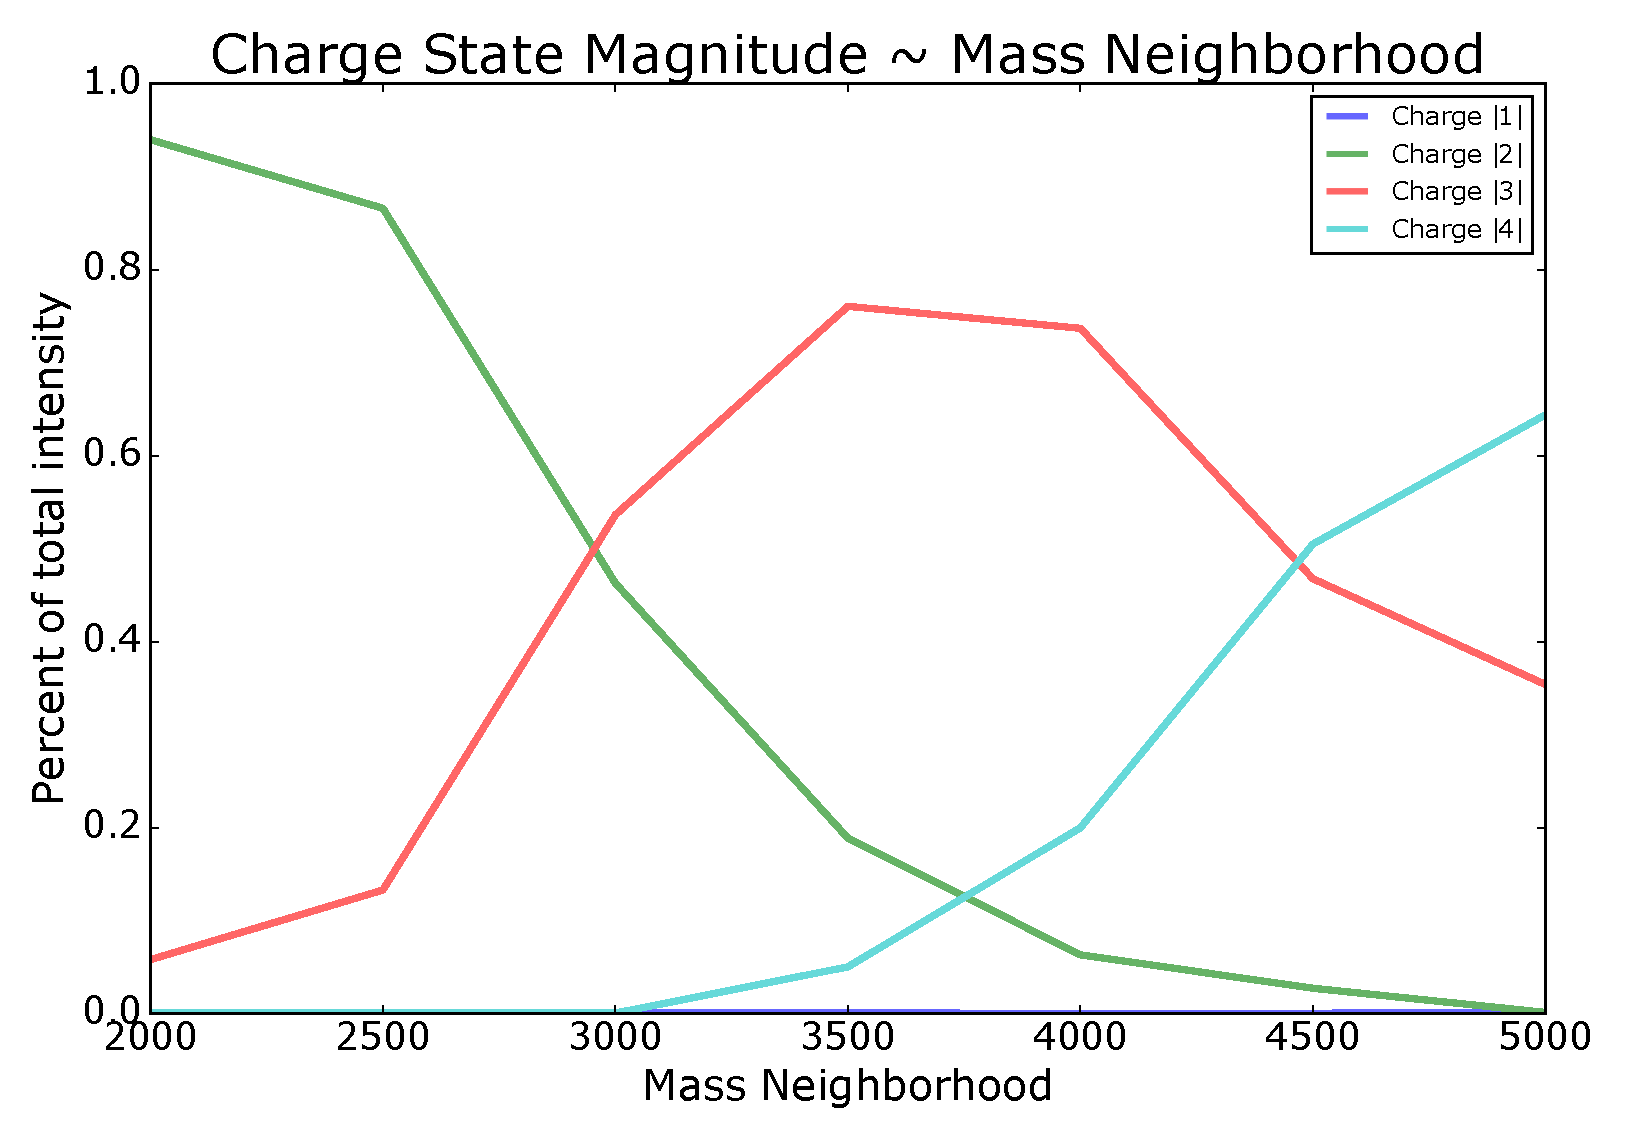
\includegraphics[width=0.75\linewidth]{figure/charge_trend_plot}
            \caption{The trend of charge state relative abundance for acidic glycans}
            \label{fig:charge_trend_plot}
        \end{figure}

    \subsubsection{Adduction Rate}
        For the samples \textit{AGP-permethylated-2ul-inj-55-SLens} and \textit{Perm-BS-070111-04-Human-Serum}
        we also include an Adduction Frequency model score $\mathscr{A}_i$, following the same
        pattern as the charge state distribution, with the same extension of justification
        from \cite{Maxwell2012}. We use one mass scaling model for all glycan compositions
        as ammmonium adduction is not expected to be composition dependent.

        \begin{align}
            \mathcal{H}_{i,j} &= \frac{
                \mathbfcal{I}_{i, a=j}}{\mathbfcal{I}_i} \nonumber\\
            P(a, m) &= |m|\sum_{m_i \in m} \mathcal{H}_{i, j} \nonumber\\
            \mathscr{A}_i &= \sum_{a_{i, j} \in \mathbf{a}_i}{P(a_{i, j}, m_i)}
        \end{align}

        We fit the adduction rate model on \textit{AGP-permethylated-2ul-inj-55-SLens} in order
        to make our comparison to third-party data less biased given limited sample data.

    \subsubsection{Isotopic Pattern Consistency}
        Our ahead-of-time deconvolution procedure uses an averagine isotopic model and does not
        capture the consistency of the isotopic pattern that was fit with the isotopic pattern
        of the glycan composition that matched that peak. The criterion
        \begin{align}
            \mathscr{I}_i &= 1 - 2\mathbfcal{I}_i^{-t}\mathbf{I}_i\sum_j^J{
                \sum_k^K{\mathcal{I}_{i, j, k}
                    \textbf{env}_{i, j, k}^t\left(
                        \ln{\textbf{env}}_{i, j, k} -
                        \ln{\textbf{tid}_{i}}
                    \right)
                }
            }
        \end{align}
        \noindent where \textbf{tid} is the theoretical isotopic pattern derived from either ${\hat g}_i$
        or an averagine interpolated for $\mathcal{M}_i$ if ${\hat g}_i =$ \O. This computes a
        per-peak intensity weighted mean G-test comparing the goodness of fit between the experimental
        envelope and the theoretical isotopic pattern.

    \subsubsection{Observation Spacing Score}
        The less time between observations of a glycan composition the less likely the chromatogram
        is to contain peaks missing or caused by isotopic pattern interference or missing information.
        \begin{align}
            \mathscr{T}_i &= 1 - 2\mathbfcal{I}_i^{-t}\mathbf{I}_i\sum_{j=1}^J\mathbfcal{I}_{i, j}(
                \mathbf{t}_{i, j} - \mathbf{t}_{i, j - 1})
        \end{align}

    \subsubsection{Summarization Score}
        Each scoring feature $\in \left[\mathscr{L}_i, \mathscr{C}_i, \mathscr{I}_i,
        \mathscr{T}_i\right]$ is penalized by $\epsilon = 1\mathrm{e}{-6}$ bounded in
        the range $[0, 1)$, with values below 0 set to $\epsilon$.

        \begin{align}
            s_i &= \sum_{f_{i,j} \in \text{features}_i}{\ln{
                \frac{f_{i, j}}{1 - f_{i, j}}
                }
            }
        \end{align}

        \noindent producing a value between $(-\infty, \infty)$. $s_i < 8$ reflects multiple
        poor feature scores and is unexpected to be real, while $s_i > 15$ is
        consistent with model expectations.

\section{$MS^n$ Signature Ion Criterion}\label{sec:signature_ion_criterion}
    When \msn scans are present, it  may be useful to consider only those \ms1
    features which are associated with \msn scans that contain glycan-like signature
    ions. We include an algorithm for classifying an \msn scan as being "glycan-like":

    \begin{align}
        I &= max(intensity(p)) \\
        t &= I * 0.01 \\
        p_{oxonium} &= \{p_i \leftarrow |ppmerror(mass(p_j), mass(f_g))| < e,
                         f_g \in oxonium(g), f_g \ne \text{Fucose}, intensity(p_i) > t\}\\
        p_{edges} &= \{(p_i, p_j) \leftarrow |ppmerror(mass(p_j) - mass(p_i), mass(f_g))| < e,\\
                  &\phantom{{}=1} oxonium(f_g) \in g , intensity(p_i) > t, intensity(p_j) > t\} \notag\\
        s_{oxonium} &= \frac{1}{|p_{oxonium}|}\sum_{p_i}^{p_{oxonium}}{
                \left(\frac{intensity(p_i)}{I}\right)
            } * min(log_4|p_{oxonium}|, 1)\\
        s_{edges} &= \frac{1}{|p_{edges}|}\sum_{p_i, p_j}^{p_{edges}}{
                \left(\frac{intensity(p_i) + intensity(p_j)}{I}\right)
            } * min(log_4|p_{edges}|, 1)\\
        s_g &= max(s_{oxonium}, s_{edges})\\
    \end{align}

    Where $p$ is the set of peaks in the scan, $g$ is the glycan compostion, $e$ the
    required parts-per-million mass accuracy. $oxonium()$ is a function that given
    a glycan composition $g$, produces fragments $f_g$ of $g$ composed of between one
    and three monosaccharides, commonly observed as oxonium ions alone, or as the mass
    difference between two peaks formed from consecutive fragmentation of a glycosidic
    bond. This method is not intended to identify a glycan structure, just detect patterns in
    the signal peaks of the \msn scan that could indicate the fragmentation of a glycan.

\section{A more complete derivation of ${\hat \phi}$}\label{sec:phi_hat_derivation}

    To obtain the optimal $\mathbf{\phi}$, we take the partial
        derivative of $\ell$ w.r.t $\phi_m$

        \begin{align}
            0 &= \frac{\partial\ell}{\partial\phi_m}\left((\mathbf{s} - \mathbf{\phi_o})^t(\mathbf{s} - \mathbf{\phi_o}) + \lambda
                \begin{bmatrix}
                    \phi_o - \tau_o, & \phi_m - \tau_m
                \end{bmatrix}
                \begin{bmatrix}
                    \mathbf{L_{oo}} & \mathbf{L_{om}} \\ \mathbf{L_{mo}} & \mathbf{L_{mm}}
                \end{bmatrix}
                \begin{bmatrix}
                    \phi_o - \tau_o \\ \phi_m - \tau_m
                \end{bmatrix}\right)\\
            &= \lambda(\phi_o - \tau_o)^t\mathbf{L_{om}} + \lambda\mathbf{L_{mo}}(\phi_o - \tau_o)
                 + \lambda(\phi_m - \tau_m)^t(\mathbf{L_{mm}}^t+ \mathbf{L_{mm}}) \nonumber\\
            &= 2\lambda\mathbf{L_{mo}}(\phi_o - \tau_o) + 2\lambda\mathbf{L_{mm}}(
                \phi_m - \tau_m) \nonumber\\
            -\mathbf{L_{mm}}(\phi_m - \tau_m) &= \mathbf{L_{mo}}(\phi_o - \tau_o) \nonumber\\
            (\phi_m - \tau_m) &= -\mathbf{L_{mm}}^{-1}\mathbf{L_{mo}}(\phi_o - \tau_o) \nonumber\\
            {\hat \phi_m} &= -\mathbf{L_{mm}}^{-1}\mathbf{L_{mo}}(\phi_o - \tau_o) + \tau_m
            \label{eqn:estimate_of_phi_m_complete}
        \end{align}

        \noindent and w.r.t. $\phi_o$

        \begin{align}
            0 &= \frac{\partial\ell}{\partial\phi_o}\left((\mathbf{s} - \mathbf{\phi_o}
                )^t(\mathbf{s} - \mathbf{\phi_o}) + \lambda
                \begin{bmatrix}
                    \phi_o - \tau_o, & \phi_m - \tau_m
                \end{bmatrix}
                \begin{bmatrix}
                    \mathbf{L_{oo}} & \mathbf{L_{om}} \\ \mathbf{L_{mo}} & \mathbf{L_{mm}}
                \end{bmatrix}
                \begin{bmatrix}
                    \phi_o - \tau_o \\ \phi_m - \tau_m
                \end{bmatrix}\right)\\
            &= -2\mathbf{s} + 2\phi_o +\lambda\left(\mathbf{L_{oo}} + \mathbf{L_{oo}}^t\right)(
                \phi_o - \tau_o) + \lambda\mathbf{L_{om}}(\phi_m - \tau_m) + \lambda\mathbf{
                L_{mo}}^t(\phi_m - \tau_m) \nonumber\\
            &= -2\mathbf{s} + 2\phi_o + 2\lambda\mathbf{L_{oo}}( \phi_o - \tau_o) + 2\lambda
                \mathbf{L_{om}}(\phi_m - \tau_m) \nonumber\\
            \mathbf{s} &= \phi_o + \lambda\left(\mathbf{L_{oo}}( \phi_o - \tau_o) +
                \mathbf{L_{om}}(\phi_m - \tau_m)\right) \nonumber\\
            &= \phi_o + \lambda\left(\mathbf{L_{oo}}( \phi_o - \tau_o) +
                \mathbf{L_{om}}(-\mathbf{L_{mm}}^{-1}\mathbf{L_{mo}}(
                \phi_o - \tau_o) + \tau_m - \tau_m)\right) \nonumber\\
            &= \phi_o + \lambda\left(\mathbf{L_{oo}}(\phi_o - \tau_o) -
                \mathbf{L_{om}}\mathbf{L_{mm}^{-1}}\mathbf{L_{mo}}(\phi_o - \tau_o)
                \right) \nonumber\\
            \mathbf{s} - \tau_o &= \phi_o - \tau_o + \lambda\left(\mathbf{L_{oo}}(\phi_o - \tau_o) -
                \mathbf{L_{om}}\mathbf{L_{mm}^{-1}}\mathbf{L_{mo}}(\phi_o - \tau_o)
                \right) \nonumber\\
            &= \mathbf{I}(\phi_o - \tau_o) + \lambda\left(\mathbf{L_{oo}}(\phi_o - \tau_o) -
                \mathbf{L_{om}}\mathbf{L_{mm}^{-1}}\mathbf{L_{mo}}(\phi_o - \tau_o)
                \right) \nonumber\\
            &= \left[
                \mathbf{I} + \lambda\left(\mathbf{L_{oo}} -
                    \mathbf{L_{om}}\mathbf{L_{mm}^{-1}}\mathbf{L_{mo}}
                \right)
            \right](\phi_o - \tau_o) \nonumber\\
            (\phi_o - \tau_o) &= \left[
                \mathbf{I} + \lambda\left(\mathbf{L_{oo}} -
                    \mathbf{L_{om}}\mathbf{L_{mm}^{-1}}\mathbf{L_{mo}}
                \right)
            \right]^{-1}(\mathbf{s} - \tau_o) \nonumber\\
            {\hat \phi_o} &= \left[
                \mathbf{I} + \lambda\left(\mathbf{L_{oo}} -
                    \mathbf{L_{om}}\mathbf{L_{mm}^{-1}}\mathbf{L_{mo}}
                \right)
            \right]^{-1}(\mathbf{s} - \tau_o) + \tau_o
            \label{eqn:estimate_of_phi_o_complete}
        \end{align}

\section{Algorithmic Performance on All Datasets}\label{sec:algorithm_performance}

\bibliographystyle{natbib}
\bibliography{bibliography}

\end{document}